\documentclass{standalone}
\usepackage{tikz}

\begin{document}

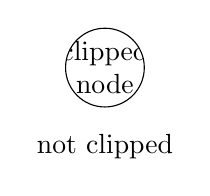
\begin{tikzpicture}
%x description="clipping"
%x code={
\begin{scope}
	\clip[draw] (0,0) circle [radius=0.50];
	\node [align=center] {clipped \\ node};
\end{scope}

\node at (0,-1) [align=center] {not clipped};
%x }
\end{tikzpicture}

\end{document}
